% 映射的同伦和空间的同伦
% 同伦|映射|空间|道路|继承|拓扑空间
%基本完成
\pentry{映射空间\upref{Topo8}}

同胚的两个拓扑空间是完全相同的,在拓扑学意义下无法区分.证明两个拓扑空间同胚通常是非常困难的,但证明两个拓扑空间不同胚却可以有很多容易计算的方法,其中一个方法就是证明两个拓扑空间不\textbf{同伦}.

同伦是一种比同胚弱一些的关系,是拓扑学中的一种代数性质.为了介绍拓扑空间中的同伦,我们首先要讨论映射的同伦.我们对于映射之间的关系和拓扑空间之间的关系都使用了“同伦”这一术语,但不会造成混淆,因为两个“同伦”之间是相互导出的概念,并且所针对的对象不同.

\subsection{映射的同伦}

\begin{definition}{映射的同伦}\label{HomT1_def1}

设有两个拓扑空间$X$和$Y$,以及它们之间的两个连续映射$f_0, f_1:X\rightarrow Y$;记$I=[0, 1]$,取度量空间$\mathbb{R}$的子空间拓扑.如果存在一个连续映射$H: X\times I\rightarrow Y$,使得对于任何$x\in X$,都有$H(x, 0)=f_0(x)$和$H(x, 1)=f_1(x)$.那么我们称$f_0$和$f_1$是\textbf{同伦}的映射,记为$f_0\overset{H}{\cong} f_1$,或者简单记为$f_0\cong f_1$;$H$称为从$f_0$到$f_1$的一个\textbf{同伦}或者\textbf{伦移}.

\end{definition}

\textbf{同伦的本质是道路.}这句话有两个含义:第一,固定$X$中的某一点$x_0$,那么$H(x_0, I)=p(I)$就是一个$I$到$Y$的映射,即一条道路;第二,在映射空间$Y^X$中来看,$f_0$和$f_1$分别是两个点,而$H$就可以看成是一个从闭区间$I$到$Y^X$上的映射,即道路.因此,我们有以下两条重要定理,一个写为习题,一个写为定理:

\begin{exercise}{映射的同伦是道路(对给定点)}\label{HomT1_exe1}
各空间和映射的定义同\autoref{HomT1_def1}.给定$x_0\in X$,对于任何的$t\in I$,构造映射$p:I\rightarrow Y$,其中$p(t)=H(x_0, t)$.证明$p$是一个连续映射,从而说明$p$是一条道路.
\end{exercise}

\begin{figure}[ht]
\centering
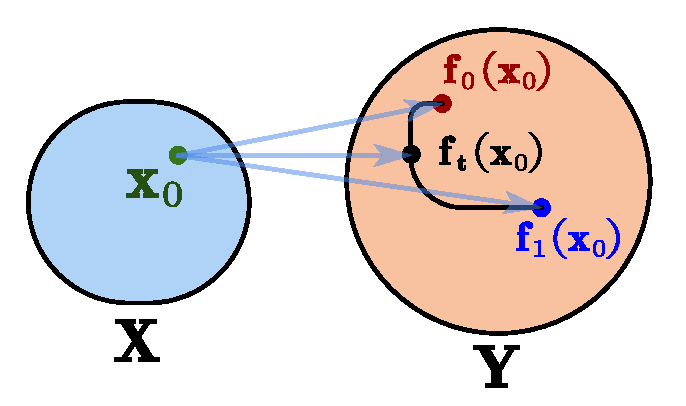
\includegraphics[width=8cm]{./figures/HomT1_1.pdf}
\caption{\autoref{HomT1_exe1} 的示意图.固定$x_0$之后,$p(t)=H(x_0, t)$在$Y$中画出一条轨迹.} \label{HomT1_fig1}
\end{figure}



\begin{theorem}{映射的同伦是道路(对同伦本身)}\label{HomT1_the1}

各空间和映射的定义同\autoref{HomT1_def1}.如果$p:I\rightarrow Y^X$满足$p(t)=f_t$,那么$p$是一个连续映射.由此可推论出,$H$本身可以看成是映射空间里的一条道路.

\end{theorem}

\textbf{证明:}

直接引用\autoref{Topo8_the1}~\upref{Topo8},令$Z=I$,$f=H$,则$p=\widetilde{f}$,因此$p$是连续映射.

\textbf{证毕.}

以上两条定理分别对于$X$中的给定点以及$X$整体的角度描述了同伦和道路的关系.第二个定理说明,两映射同伦,等价于说两映射是同一条道路的两端,还等价于说两映射是同一条道路上的两点.由于道路可以首尾相接从而得到新的道路,因此同一个映射空间中,如果$f\cong g$而$g\cong h$,那么一定有$f\cong h$.这就是说,同伦关系是具有传递性的.考虑到同伦关系显然还有自反性和对称性,我们直接可得如下定理:

\begin{theorem}{}
映射的同伦关系是一个等价关系.
\end{theorem}

映射之间还有复合运算,同伦关系也会继承到复合运算上.

\begin{theorem}{映射同伦关系的继承}\label{HomT1_the2}

设$X$,$Y$和$Z$是三个拓扑空间,$f_0, f_1:X\rightarrow Y$,$g_0, g_1:Y\rightarrow Z$分别是连续映射,且有$f_0\overset{F}{\cong}f_1$和$g_0\overset{G}{\cong}g_1$.那么$g_0\circ f_0\cong g_1\circ f_1$.

\end{theorem}

\textbf{证明:}

由于$F:X\times I\rightarrow Y$和$g_0:Y\rightarrow Z$都是连续映射,故$g_0\circ F:X\times I\rightarrow Z$是一个连续映射,故$g_0\circ F$是一个连接了$g_0\circ f_0$和$g_0\circ f_1$的道路.故$g_0\circ f_0\cong g_0\circ f_1$.

类似地,$G\circ(f_1\times 1_I):X\times I\rightarrow Z$\footnote{$1_I:I\rightarrow I$是恒等映射,$f_1\times 1_I$的定义见乘积拓扑\upref{Topo6}中的\autoref{Topo6_exe1}.}是一个连接了$g_0\circ f_1$和$g_1\circ f_1$的道路,故$g_0\circ f_1\cong g_1\circ f_1$.

综上,由映射同伦的传递性,$g_0f_0\cong g_1f_1$.

\textbf{证毕.}

\subsection{拓扑空间的同伦}

\begin{definition}{空间同伦}

设有两个拓扑空间$X$和$Y$,如果存在连续映射$f:X\rightarrow Y$和$g:Y\rightarrow X$,使得$gf\cong 1_X$且$fg\cong 1_Y$,那么我们称$X$和$Y$是\textbf{同伦}的,或者说\textbf{具有相同的伦型}.$f$称为从$X$到$Y$的\textbf{同伦等价},反过来$g$是从$Y$到$X$的同伦等价,二者互为\textbf{同伦逆}.

\end{definition}

同伦和同胚一样,也是一个等价关系,只是要更弱一些,使得不同胚的空间也有可能同伦.当然,同胚的空间必然同伦.

\begin{exercise}{}
证明空间的同伦具有传递性,从而推论同伦是一个等价关系.
\end{exercise}

\subsection{思考}

在映射空间\upref{Topo8}中所定义的紧开拓扑看起来很不接地气.本小节\autoref{HomT1_exe1} 直观地阐释了同伦的意义,即对于每个固定点$x_0\in X$,同伦$H$都会在$Y$中画出一条道路,这意味着每个点的映射都是\textbf{连续地变化}的.\autoref{HomT1_the1} 说明,整体上来看,$H$本身是映射空间$Y^X$中的一条道路.从这个联系来看,思考一下为什么要用紧开拓扑来定义映射空间.

